%% report/jsa/paper.tex
%% Elsevier (elsarticle) manuscript for the Journal of Systems Architecture.
%% report/elsevier/README.md lists the commands that regenerate the numbers.

\documentclass[preprint,12pt]{elsarticle}

\usepackage{amsmath,amssymb}
\usepackage{graphicx}
\usepackage{booktabs}
\usepackage{longtable}
\usepackage{array}
\usepackage{multirow}
\usepackage{adjustbox}
\usepackage{needspace}
\usepackage[hyphens,obeyspaces,spaces]{url}
\usepackage{hyperref}
\usepackage{xcolor}
\usepackage{tikz}
\usetikzlibrary{arrows.meta,positioning,shapes.geometric,fit,backgrounds,patterns}

\newcommand{\cfgA}{Config~A}
\newcommand{\cfgB}{Config~B}
\newcommand{\cfgC}{Config~C}
\newcommand{\ttc}{TT\&C}
\DeclareUrlCommand\code{\urlstyle{tt}}
\newcommand{\TestCount}{1,218}

\journal{Journal of Systems Architecture}

\setlength{\emergencystretch}{3em}
\begin{document}

\begin{frontmatter}

\title{Configuration-driven mode logic for resource-constrained embedded systems: requirement-based model checking, torn-write persistence and a PocketQube case study}
\author{Nikunj Rathi\corref{cor1}}
\ead{nikunj.rathi@somaiya.edu}
\cortext[cor1]{Corresponding author}
\author{Purva Pote}
\ead{purva.pote@somaiya.edu}
\author{Megha Sharma}
\ead{meghasharma@somaiya.edu}
\affiliation{organization={K. J. Somaiya School of Engineering, Somaiya Vidyavihar University},
            city={Mumbai},
            country={India}}
\begin{abstract}
This paper describes a state-machine engine for embedded mode logic that keeps every mission constant out of the code. States, events, guarded transitions, persisted latches and event-conflict ranks are YAML data checked against one schema, and the C transition table and a TLA+ specification are generated from the same file. That shared file is also a risk, because a check derived from it can repeat its errors. In a study of 288 configuration mutants, TLC with properties derived from the file killed only the 18 that the loader already rejects. All checks together, including hand-written requirement properties and threshold-boundary tests, killed 96.1\% of the 256 non-equivalent mutants. Under a model in which any save can be torn by a reset, the hand-written properties found a path that bypassed a persisted latch. Review found a second defect, a latch held by only one of two non-volatile banks until the next save, and counting flash writes showed that saving on every legal step would wear the banks out in about 52~h. A save now writes only when the content changes, and then writes both banks. Three PocketQube lifecycles run on the engine without code changes. A C port on an emulated STM32F401RE under Zephyr reproduced all 35,763 decisions of a 48~h trace in 36,728~B of flash and 11,648~B of RAM. Timing and power were not measured.
\end{abstract}

\begin{keyword}
finite-state machine \sep embedded software \sep model checking \sep TLA+ \sep mutation testing \sep non-volatile memory \sep PocketQube
\end{keyword}

\end{frontmatter}

% =====================================================================
\section{Introduction}\label{sec:intro}
% =====================================================================

This work started from a flight-software problem. A PocketQube is a picosatellite built from 5~cm cubic units that typically averages under 1~W~\cite{Franzese2025Survey}, and its software has to confirm that it has left the deployer before radiating, respect a radio-silence period, drop into a safe mode on faults or low charge, accept ground overrides at any time, and come back to a legal state after an arbitrary reset without forgetting that deployment was already confirmed. The project reported here had neither hardware nor an interface-control document (ICD), so timer durations, battery thresholds and link margins were unknown when the mode logic had to be designed.

The response was to treat every such value as data with a recorded source and confidence, and to keep the engine that interprets that data free of mission constants. A new mission then edits a configuration file and a parameter table. The use case added one governance constraint: nothing happens on board unless it was uplinked or triggered by the system's own safe-mode logic, and a ground operator can override the autonomous behaviour at any time.

Moving the logic into data creates a verification problem. One YAML file feeds the engine, the model checker and the firmware table, so a check derived from that file can pass on an error the file contains. Persistence raises a second problem. A mode machine's guarantees depend on what survives a reset, and a reset can arrive in the middle of a non-volatile write.

The work addresses four questions. RQ1: can one engine drive structurally different lifecycles with no code changes? RQ2: does the engine stay in a legal state, and keep a persisted latch, across arbitrary resets including resets in the middle of a non-volatile write? RQ3: how much of each check depends on the configuration file it is meant to check? RQ4: does the decision logic survive a port to C on a microcontroller target with identical behaviour, and at what memory cost?

The contributions are as follows.
\begin{enumerate}
\item A YAML schema with a guard grammar and a closed-world rule for undefined state--event pairs, interpreted by an engine with no mission constants, with conflict-ranked event arbitration, A/B-bank persistence and optional HMAC-SHA256 command authentication (Section~\ref{sec:design}).
\item A configuration-mutation study that measures how many errors each check catches when the check shares its source with the code, set beside tests, reset and corruption injection, and TLC model checking of hand-written requirement properties (Section~\ref{sec:verification}).
\item Persistence defects found by these checks, by review and by counting flash writes, the fix for each, and a case-by-case statement of what the persistence layer guarantees under one fault at a time (Sections~\ref{sec:persistence} and~\ref{sec:mc}).
\item A C port checked call for call against the Python engine on an emulated Cortex-M4 under Zephyr, with its memory footprint (Section~\ref{sec:cport}).
\item A case study of three PocketQube lifecycles (Section~\ref{sec:configs}), exercised in a simulation built on the published figures of the POQUITO mission (Section~\ref{sec:sim}).
\end{enumerate}

The engine decides; it does not drive hardware. Actions such as \code{enable_rf} are logged, not executed, and nothing here is flight-qualified. Results are labelled by where they come from: the configurations and tests, the TLA+ model, the emulated firmware, or the simulation (Table~\ref{tab:scope}).

% =====================================================================
\section{Related work}\label{sec:related}
% =====================================================================

\paragraph{State machines and synchronous languages} Statecharts~\cite{Harel1987Statecharts} established hierarchical state machines as a design notation for reactive systems, and Esterel~\cite{Berry1992Esterel} gave reactive control a synchronous language with a formal semantics. The configurations here are flat machines with latches and guards, closer to what a microcontroller can interpret from a table.

\paragraph{Model checking} Model checking of finite-state systems against temporal properties goes back to Clarke et al.~\cite{Clarke1986ModelChecking}, and SPIN~\cite{Holzmann1997SPIN} brought it into routine use for protocols and flight software. The model checking of Section~\ref{sec:verification} uses TLA+~\cite{Lamport2002TLA} and its explicit-state checker TLC~\cite{Yu1999TLC}; Newcombe et al.~\cite{Newcombe2015AWS} report the same toolchain finding design errors in industrial systems that testing had missed.

\paragraph{Mutation analysis} Mutation testing seeds small faults and counts how many a test suite detects; Jia and Harman~\cite{Jia2011Mutation} survey the field. The study in Section~\ref{sec:verification} applies the idea to configuration data rather than program text, and uses it to compare checks that share a source with checks that do not.

\paragraph{Flight-software structure and fault management} The ECSS operability standard~\cite{ECSS2008Operability} sets requirements for on-board fault detection, isolation and recovery (FDIR) and for ground observability and control. Latachi et al.~\cite{Latachi2020Masat} describe reusable flight-control software for the Masat-1 CubeSat with a watchdog and mode-based safe handling; the framework's watchdog timeout follows their pattern. Eshaq et al.~\cite{Eshaq2025CubeSatFSW} present a CubeSat flight-software case study whose watch-point and action-point fault handling avoids reacting to a single event, which motivated the three-consecutive-fault threshold used here. Dependability vocabulary follows Avi\v{z}ienis et al.~\cite{Avizienis2004Dependability}, and software fault injection follows the survey of Hsueh et al.~\cite{Hsueh1997FaultInjection}.

\paragraph{Persistence and memory faults} A NASA NEPP assessment~\cite{Murphy2022NEPP} measures how much of the fault space the memory test patterns used on flight parts cover and finds gaps, and a JPL guideline on MNOS EEPROM in space~\cite{Chen2006EEPROM} reports weak-cell and retention problems in flight parts. Both argue for persistence that tolerates a corrupted or half-written record. The engine uses two banks, CRC-32 and a sequence number; Koopman and Chakravarty~\cite{Koopman2004CRC} discuss CRC polynomial choice for embedded networks.

\paragraph{Small-satellite case study} Franzese's survey~\cite{Franzese2025Survey} collects the PocketQube missions flown so far. The POQUITO mission's system-design paper~\cite{Franzese2026POQUITO} gives the battery, generation, downlink and timer figures that the case study adopts. Villela et al.~\cite{Villela2019Thousandth} estimate the CubeSat mission success rate at about 75\% once launch failures are excluded, which is one reason the design concentrates on deployment confirmation and reset behaviour.

The authors are not aware of prior work that combines a mission-agnostic configuration schema for lifecycle mode logic, model checking of specifications generated from that schema, a mutation study of how far those checks depend on the schema instance, and a call-level equivalence check of an embedded port. Each piece exists separately in the works above.

% =====================================================================
\section{Engine design}\label{sec:design}
% =====================================================================

\subsection{Architecture}

The engine (Fig.~\ref{fig:architecture}) has seven parts: a transition-table interpreter, a guard evaluator, an event arbiter, a priority-queue scheduler, an A/B-bank persistence layer, a decision logger and a fault-injection harness. The interpreter's entry point, \code{step(config, state, event, context)}, returns the new state and a list of actions. It is written in Python; the engine, simulation and policy packages together are about 4,600 lines. The engine package itself is about 1,300 lines and contains no mission constants. The simulation consumes the engine's decisions and produces delivery, latency and energy metrics; the C port of Section~\ref{sec:cport} uses a table generated from the same configuration file.

\begin{figure}[t]
\centering
\resizebox{\textwidth}{!}{%
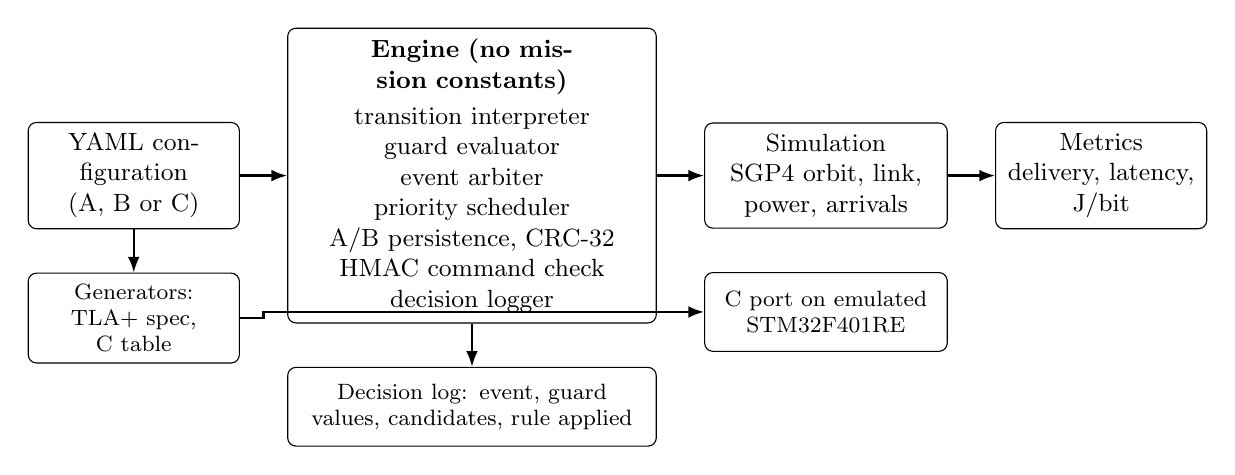
\begin{tikzpicture}[
  box/.style={draw, rounded corners=3pt, minimum height=1.0cm, align=center, font=\small, inner sep=4pt},
  arr/.style={-{Latex[length=2mm]}, thick}]
\node[box, text width=2.4cm] (cfg) {YAML configuration\\(A, B or C)};
\node[box, text width=4.4cm, right=0.6cm of cfg, minimum height=2.4cm] (engine)
  {\textbf{Engine (no mission constants)}\\[2pt] transition interpreter\\ guard evaluator\\ event arbiter\\ priority scheduler\\ A/B persistence, CRC-32\\ HMAC command check\\ decision logger};
\node[box, text width=2.8cm, right=0.6cm of engine] (sim) {Simulation\\SGP4 orbit, link,\\power, arrivals};
\node[box, text width=2.4cm, right=0.6cm of sim] (out) {Metrics\\delivery, latency,\\J/bit};
\node[box, text width=4.4cm, below=0.55cm of engine, font=\footnotesize] (log) {Decision log: event, guard values, candidates, rule applied};
\node[box, text width=2.4cm, below=0.55cm of cfg, font=\footnotesize] (gen) {Generators: TLA+ spec, C table};
\node[box, text width=2.8cm, below=0.55cm of sim, font=\footnotesize] (c) {C port on emulated STM32F401RE};
\draw[arr] (cfg) -- (engine); \draw[arr] (engine) -- (sim); \draw[arr] (sim) -- (out);
\draw[arr] (engine) -- (log); \draw[arr] (cfg) -- (gen); \draw[arr] (gen.east) -- ++(0.3,0) |- (c.west);
\end{tikzpicture}}
\caption{Framework architecture. The configuration file is the only mission-specific input; the TLA+ specification and the C transition table are generated from it.}
\label{fig:architecture}
\end{figure}

\subsection{Configuration schema}

A configuration has nine top-level keys: \code{meta}, \code{states}, \code{events}, \code{transitions}, \code{parameters}, \code{latches}, \code{data_class_priority}, \code{conflict_resolution} and \code{mode_exclusivity_groups}. A state has an identifier, name, documentation category, entry actions and an initial-state flag. An event has an identifier, a name and a source tag (\code{onboard}, \code{ground}, \code{scheduler} or \code{harness}). A transition has an identifier, a \code{from} list (or \code{"*"} for every state), an event, an optional guard, a target and a list of actions and requirement identifiers. The target is a state, \code{null} for a self-loop that only logs, or \code{reload_from_persistence}. Latches are declared once at top level with the transitions that set them and whether they survive a reset, so their semantics are not scattered across state entries.

\paragraph{Closed-world rule} A state--event pair with no matching transition, after expanding \code{"*"} and multi-state \code{from} lists and after evaluating guards, is illegal. The engine resolves it to a no-op: the state is unchanged, no action fires, and the decision log records the illegal pair. The rule belongs to the schema contract, so no configuration restates it.

\paragraph{Guards} Every guard in the three shipped configurations is a single binary comparison:
\begin{verbatim}
guard    ::= operand op operand
op       ::= "==" | "!=" | ">=" | "<=" | "<" | ">"
operand  ::= "context." ID | ID | PARAM_ID
           | "elapsed(" ID ")" | literal
PARAM_ID ::= /P[BC]?-\d{3}/
\end{verbatim}
\code{context.*} names refer to engine state that persists between steps and that only actions change. Bare identifiers such as \code{battery_soc} or \code{elevation} are telemetry supplied fresh on each step, which the engine reads but never writes. Boolean combinators are not implemented because no configuration needs them yet.

\paragraph{Actions} An action is either a context assignment (\code{set context.x = v}), which the engine applies, or an opaque identifier such as \code{enable_rf}, which the engine logs and does not execute. Wiring opaque actions to hardware is outside this software-only project; the decision log is the evidence that the correct action would have fired.

\subsection{Event conflict resolution and data-class priority}

Two orderings answer different questions and live under different keys. The data-class priority (\ttc{} $>$ SSTV $>$ Codec2/M17) is fixed by the mission's governance table and tells the scheduler which queued item to send next. The conflict-resolution ranking tells the arbiter which of several pending events to service first in one tick (Table~\ref{tab:conflict}). It is a configuration choice.

\begin{table}[t]
\centering
\small
\caption{Event conflict-resolution ranks shared by the three configurations.}
\label{tab:conflict}
\adjustbox{max width=\textwidth}{\begin{tabular}{@{}clp{0.48\textwidth}@{}}
\toprule
Rank & Category & Tie-break within the rank \\
\midrule
1 & Ground override, reset & Earliest timestamp; \code{RESET} wins ties against ground commands \\
2 & Fault, watchdog, power, comms loss & Timestamp, then event identifier \\
3 & Deployment lifecycle & Timestamp \\
4 & Scheduler, pass end & Data-class priority; \code{PASS_END} before any \code{SCHEDULER_SELECT_*} \\
5 & Routine & Timestamp \\
\bottomrule
\end{tabular}}
\end{table}

The arbiter sorts the pending events by rank, then by a data-class key within the scheduler rank (\code{PASS_END} before any select, selects in data-class priority order), then by timestamp, then with \code{RESET} ahead of other rank-1 events at an equal time, and finally by event identifier. The tie-break rule for each rank is read from the configuration's tie-break text, and text the arbiter does not recognise is a load error. It services the highest-ranked event that has a legal transition, drops higher-ranked events that have none, and keeps the rest queued with their original timestamps for the next tick. The step function itself still takes one event. The ranking matters for logging as well as for behaviour. When a ground safe-mode command and a natural pass end arrive in the same tick, the ground command is serviced, the pass end stays queued, and the log records a ground override with the queued event named.

A ranking that is only validated has no effect, so the simulation driver routes every tick through the arbiter. With a fixed trial order, a safe-mode state would try autonomous recovery (rank~2) ahead of a ground exit (rank~1).

\subsection{Persistence and decision log}\label{sec:persistence}

The engine calls save after every legal step, and a save whose content both banks already hold writes nothing. A save that changes the content writes a record to the bank not holding the newest valid record, then writes it to the other bank with the next sequence number. A bank that already holds the content is not rewritten, so a damaged or stale bank is repaired by the next save with one write. A record holds the state and context, a sequence number taken from the newest valid bank, and a CRC-32 over the sequence and the body. At boot both banks are read, a bank whose CRC fails is skipped whatever its sequence number, and the valid bank with the higher sequence number is loaded. A record is committed when its save returns, and from then on both banks hold it. In C, a failed first write stops the second, which would otherwise erase the good copy.

The fault model is one fault at a time: a reset at any point, including in the middle of a write, or corruption of one bank's contents. Table~\ref{tab:persist} lists the cases. Writing both banks closes a window in which a new record would be held only by the bank just written until the following change, so that corruption of that bank reloads the older record, which may lack a newly set latch or repeat an action that only a latch guards. An earlier design mirrored only latch-setting saves. It has half the wear, but the fault-injection sweep showed that corrupting the newest bank then rolls the state back one transition.

Review of the write-on-change design found three defects in bank selection. Taking the target as the bank not written last could overwrite the only good copy, because a torn record has a readable sequence and looks newest, so two resets in a row lost everything. The next sequence was read from every bank, valid or not, and a torn erase can leave a value near the top of the 32-bit range. The sequence field lay outside the CRC, so a tear of that field alone left a CRC-valid record with a garbage sequence and a stale record could win; a power-cut harness found this one in the first version of the fix. The target and the sequence now come from valid banks only, and the CRC covers the sequence.

\begin{table}[t]
\centering
\footnotesize
\caption{Persistence outcomes under one fault at a time.}
\label{tab:persist}
\begin{tabular}{@{}p{0.45\textwidth}p{0.47\textwidth}@{}}
\toprule
Fault & Outcome \\
\midrule
Reset during the first write of a change & Older record loads; a latch in the new record is not committed and deployment is confirmed again \\
Reset during the second write & The first copy is valid and is the new record \\
Corruption of either bank after a save returns & The other bank restores the same record; the next save repairs the damaged bank \\
Torn erase or program, with a garbage sequence & Bank invalid; ignored by load, target choice and the sequence counter \\
Bit flip in a sequence field & Bank invalid \\
Reset again on the next write & The only valid bank is never the target, so it survives \\
Corruption of both banks, or corruption plus a reset during one save (two faults) & Out of scope; with both banks corrupted the engine starts from the initial state with an empty context and the latch is lost \\
\bottomrule
\end{tabular}
\end{table}

The decision log records every transition, including illegal-pair no-ops, with the triggering event and guard inputs, and every scheduler choice with the competing candidates and the rule that decided. The verification-matrix generator reads this log and the test results to map requirements to evidence.

\subsection{Ground-command authentication}\label{sec:auth}

Every event carries a source tag. Ground-sourced events can be signed with HMAC-SHA256~\cite{RFC2104,Bellare1996HMAC,NIST2015SHS} over the event identifier and timestamp, and signatures are compared in constant time. With \code{require_auth}, a missing secret is a configuration error that stops the engine before any transition is evaluated, and a missing, forged or wrong-key signature makes the event illegal whatever its guard would have said. With \code{replay_protection}, each command also carries a signed counter that is stored in the persisted context; a verified counter is consumed even if the command's guard then fails, so a rejected command cannot be replayed later when the guard would pass. The counter does not survive a cold start with no valid record, and a test pins that limit.

With no secret the engine does not read the source tag, and every experiment in this paper uses that mode. The C port verifies the two-field message without the counter, so replay protection exists in the Python engine only. Key provisioning and rotation, link-layer protection as in CCSDS SDLS~\cite{CCSDS2022SDLS} and a freshness window are out of scope.

% =====================================================================
\section{Case study: three PocketQube configurations}\label{sec:configs}
% =====================================================================

\subsection{Config A: PocketQube reference}

\cfgA{} instantiates all three deployment mechanisms named in the use case: a separation switch, an RF-inhibit timer and an independent RF-beacon path. Both confirmation paths must agree before the one-way \code{deployment_confirmed} latch is set. The configuration has 10 states, 20 events and 24 transitions traced to 34 requirements (Fig.~\ref{fig:config-a}; the full table is in~\ref{app:trans-a}). The four downlink modes (\ttc{}, SSTV, voice, idle) are separate, mutually exclusive states.

\begin{figure}[t]
\centering
\resizebox{\textwidth}{!}{%
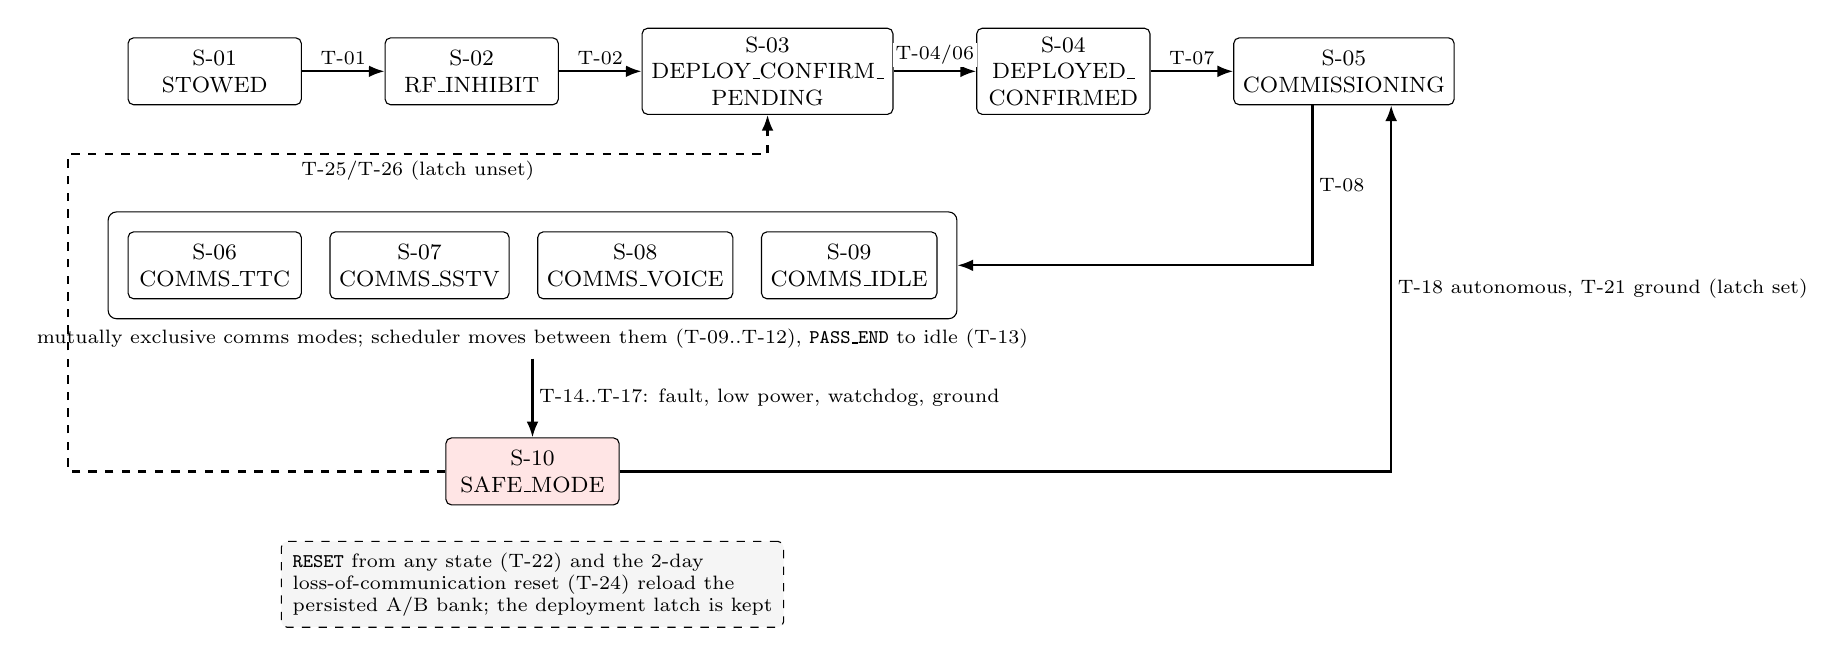
\begin{tikzpicture}[
  st/.style={draw, rounded corners=2pt, minimum height=0.85cm, minimum width=2.2cm, align=center, font=\footnotesize},
  saf/.style={st, fill=red!10},
  note/.style={draw, dashed, rounded corners=2pt, align=left, font=\scriptsize, fill=gray!8, inner sep=4pt},
  arr/.style={-{Latex[length=2mm]}, thick},
  lab/.style={font=\scriptsize, fill=white, inner sep=1pt}]
\node[st] (s1) {S-01\\STOWED};
\node[st, right=1.05cm of s1] (s2) {S-02\\RF\_INHIBIT};
\node[st, right=1.05cm of s2] (s3) {S-03\\DEPLOY\_CONFIRM\_\\PENDING};
\node[st, right=1.05cm of s3] (s4) {S-04\\DEPLOYED\_\\CONFIRMED};
\node[st, right=1.05cm of s4] (s5) {S-05\\COMMISSIONING};
\node[st, below=1.6cm of s1] (s6) {S-06\\COMMS\_TTC};
\node[st, right=0.35cm of s6] (s7) {S-07\\COMMS\_SSTV};
\node[st, right=0.35cm of s7] (s8) {S-08\\COMMS\_VOICE};
\node[st, right=0.35cm of s8] (s9) {S-09\\COMMS\_IDLE};
\begin{scope}[on background layer]
\node[draw, rounded corners=3pt, fit=(s6)(s9), inner sep=7pt, label={[font=\scriptsize]below:mutually exclusive comms modes; scheduler moves between them (T-09..T-12), \texttt{PASS\_END} to idle (T-13)}] (comms) {};
\end{scope}
\node[saf, below=1.5cm of comms] (s10) {S-10\\SAFE\_MODE};
\node[note, below=0.45cm of s10] (bank) {\texttt{RESET} from any state (T-22) and the 2-day\\loss-of-communication reset (T-24) reload the\\persisted A/B bank; the deployment latch is kept};
\draw[arr] (s1) -- node[lab, above=1pt]{T-01} (s2);
\draw[arr] (s2) -- node[lab, above=1pt]{T-02} (s3);
\draw[arr] (s3) -- node[lab, above=1pt]{T-04/06} (s4);
\draw[arr] (s4) -- node[lab, above=1pt]{T-07} (s5);
\draw[arr] ([xshift=-4mm]s5.south) |- node[lab, pos=0.25, right=1pt]{T-08} (comms.east);
\draw[arr] (s10.north -| comms.south) ++(0,1.0) -- node[lab, right=1pt]{T-14..T-17: fault, low power, watchdog, ground} (s10.north);
\draw[arr] (s10.east) -| node[lab, pos=0.75, right=1pt]{T-18 autonomous, T-21 ground (latch set)} ([xshift=6mm]s5.south);
\coordinate (lane) at ([xshift=-5mm]comms.west);
\coordinate (top) at ([yshift=-5mm]s3.south);
\draw[arr, dashed] (s10.west) -| (lane) |- node[lab, pos=0.75, below=1pt]{T-25/T-26 (latch unset)} (top) -- (s3.south);
\end{tikzpicture}}
\caption{Simplified \cfgA{} lifecycle. Safe-mode entries (T-14..T-17) also leave from COMMISSIONING and, for the ground command, from S-03 onward. Safe-mode exits return to commissioning only when the deployment latch is set and otherwise to S-03. The full transition table is in~\ref{app:trans-a}.}
\label{fig:config-a}
\end{figure}

\cfgA{} lets the satellite leave safe mode on its own once recovery conditions hold (T-18), with a 15-percentage-point hysteresis between the 25\% entry and 40\% recovery charge thresholds to stop chattering. A ground operator can force or hold safe mode from S-03 onward (T-17) and can force an exit (T-21). Both exits are guarded on the deployment latch. A safe-mode episode entered from S-03 before confirmation returns to S-03 (T-25, T-26), keeping any confirmation path that had already asserted.

\subsection{Config B: single path, single mode}

\cfgB{} was written directly against the schema, before any engine existed, to test whether the schema could express a different mission without new fields. It differs from \cfgA{} on five axes (Table~\ref{tab:axes}): it confirms deployment from the switch and a debounce timer alone, has no RF-inhibit timer, has one downlink mode, and leaves safe mode only on a ground command. It has 7 states, 15 events, 15 transitions and 12 requirements. No schema change was needed: the schema has no minimum counts, a two-member mode-exclusivity group is legal, and removing autonomous recovery means leaving out the event and transition.

\subsection{Config C: the remaining axis combination}

\cfgA{} pairs dual-path deployment with autonomous recovery and \cfgB{} pairs single-path deployment with ground-only recovery. \cfgC{} adds single-path deployment with autonomous recovery: \cfgB{}'s seven-state structure plus an autonomous exit (T-16) next to the retained ground exit (T-12), for 16 transitions and 13 requirements. The simulation driver's recovery logic looks the recovery threshold up by parameter name, so it drove \cfgC{} without modification. \cfgC{} is synthetic. It is excluded from the policy comparison and uses the two-station scenario of Section~\ref{sec:sim} as its reference. The fourth combination, dual-path deployment with ground-only recovery, is not built.

\begin{table}[t]
\centering
\small
\caption{Structural differences between the three configurations.}
\label{tab:axes}
\adjustbox{max width=\textwidth}{\begin{tabular}{@{}lccc@{}}
\toprule
Axis & \cfgA{} & \cfgB{} & \cfgC{} \\
\midrule
Deployment confirmation & Switch+timer and beacon & Switch+debounce & Switch+debounce \\
RF-inhibit timer & 900~s & None & None \\
Downlink-mode states & 4 & 1 (+ idle) & 1 (+ idle) \\
Safe-mode exit & Autonomous or ground & Ground only & Autonomous or ground \\
States / events / transitions & 10 / 20 / 24 & 7 / 15 / 15 & 7 / 16 / 16 \\
Requirements & 34 & 12 & 13 \\
Parameters in YAML & 20 & 15 & 15 \\
\bottomrule
\end{tabular}}
\end{table}

\subsection{Defects found in design review}

A review held before the engine was written found five blocking defects. \cfgB{}'s deployment sequence deadlocked, because its only transition tested an elapsed-time guard on a timer that nothing started; the fix split it into an arm step and a check step. The schema did not list \code{to: null} as legal although both configurations used it. One \cfgA{} event was missing from the conflict ranking. The deployment-confirmation timeout parameters were declared but no guard read them, so a confirmation path that never asserted had no escalation; the fix extended the ground safe-mode transition to the deployment-pending states. The two parameters (P-011, P-012) are still read by no guard, because leaving the pending state on a single unconfirmed signal would be unsupervised autonomy. Model checking later found that this fix had opened a path to commissioning without the latch (Section~\ref{sec:mc}). Finally, a ground-only safe-mode exit branch in \cfgA{} could never be reached and was deleted.

\subsection{Parameter governance}

Every numeric guard value not fixed by the use case is a parameter with a source and a confidence of \code{cited}, \code{assumed} or \code{tbd}, and every assumed value carries a written justification. The register lists 21 \code{P-} parameters, of which 20 appear in the \cfgA{} YAML; the exception, P-021 (the A/B bank-swap policy), is an engine-level policy shared by all configurations. \cfgB{} and \cfgC{} use separate identifier namespaces (\code{PB-}, \code{PC-}) so that no reader assumes a value is shared.

% =====================================================================
\section{Verification}\label{sec:verification}
% =====================================================================

\subsection{Test suite and fault injection}

For each configuration, the suite runs every transition row as a positive case and every state--event pair absent from the table as a no-op assertion. Every guarded row also has a guard-false case and a case at the threshold, with the inclusive or exclusive side taken from the requirement wording. Resets are injected at every transition boundary and, separately, at every byte boundary of a simulated non-volatile write, in the style of software-implemented fault injection~\cite{Hsueh1997FaultInjection}. Persistence tests corrupt either bank after every save history of up to five saves, and a random walk over each configuration injects resets and corrupts either bank at random, including straight after the step that sets the latch; none may clear \code{deployment_confirmed} once its save has returned. A cross-configuration harness asserts three engine-level guarantees on every configuration: latch integrity (R-04, RB-02, RC-02), ground override from the RF-enabled states onward (R-22, RB-08, RC-08), and legality of \code{RESET} from every state with latch survival (R-27/R-29, RB-10, RC-10).

The suite has \TestCount{} passing tests. Statement coverage of the engine is 96.9\% and branch coverage 91.9\%. The verification matrix maps 34 \cfgA{}, 12 \cfgB{} and 13 \cfgC{} requirements to tests, and separates a requirement that a test merely names from one whose test result was recorded as an executed pass.

\subsection{Model checking}\label{sec:mc}

Tests enumerate cases chosen by people. To cover every reachable state, a generator writes a TLA+ module and TLC configuration from each YAML file on every run. The module tracks the control state, the latch, the Boolean context flags and a snapshot of these that stands for the last completed save. Every step either saves or leaves the previous snapshot in place, as a torn write would, and a reset restores the snapshot as the engine does. The two banks are abstracted into that one snapshot, so the model covers torn saves but not later corruption of a completed bank; a separate two-bank model, described below, covers that case. Guards that compare a Boolean context flag are encoded exactly. All other guards (timers, telemetry, parameters) are nondeterministic, which over-approximates the reachable behaviour.

TLC~\cite{Yu1999TLC} checks properties of two kinds. Generic ones come from the configuration: \code{TypeOK}, the persisted latch never clears, and once persisted the live latch is set. The others are written by hand from the requirements documents, naming states and events rather than reading them from the YAML: the latch rises only on the declared confirmation events (for \cfgA{}, only once both paths have confirmed); the RF-silent states are left only when the inhibit or debounce timer expires; safe mode is entered and left only through the declared events; ground safe-mode entry is available from exactly the RF-enabled states; reset is always available; and commissioning and every downlink state require the latch. Deadlock checking stays on.

The first run of this model found a defect in \cfgA{}. A ground safe-mode command from the confirmation-pending state, followed by either safe-mode exit, reached commissioning and then nominal downlink with the latch unset, in breach of the requirement that commissioning begins only after the latch is set. The engine reproduced the trace. It came from the design-review fix of Section~\ref{sec:configs}, which let T-17 start from the pending states while both exits still went to commissioning. Both exits are now guarded on the latch, and two new rows return an unlatched satellite to the pending state. After the fix all three configurations satisfy every property (Table~\ref{tab:tlc}).

The in-RAM form of the latch property is false in this model, and the checker script asserts that it stays false so that the persistence model cannot silently become vacuous: a reset that tears the save of the latch-setting step reloads the older bank. The model says nothing about timing, thresholds or liveness.

A hand-written module does the opposite of the generated ones. The mission shrinks to three contents, and the model keeps both banks, each erase and program step, a reset at any point, torn records with readable sequences, and corruption of one bank while no save is running. Its invariants state that a committed record stays loadable, a load is never older than the last commit, a committed latch is never lost, and a save that returns leaves both banks holding the record. TLC finds no violation in 3,690 distinct states, and three protocol mutants (a target chosen by raw sequence, a single write per change, and a save skipped when either bank holds the content) must each violate an invariant. Corruption during a save is a double fault and is left out, and neither wear nor time is modelled.

\begin{table}[t]
\centering
\small
\caption{TLC 2.19 results with the persistence model, after the \cfgA{} fix.}
\label{tab:tlc}
\adjustbox{max width=\textwidth}{\begin{tabular}{@{}lrrrrl@{}}
\toprule
Configuration & Declared states & States generated & Distinct states & Depth & Result \\
\midrule
\cfgA{}, before the fix & 10 & 41 & 16 & 4 & Latch-before-commissioning violated \\
\cfgA{} & 10 & 7,657 & 434 & 11 & No error \\
\cfgB{} & 7 & 1,798 & 121 & 9 & No error \\
\cfgC{} & 7 & 1,991 & 128 & 9 & No error \\
\bottomrule
\end{tabular}}
\end{table}

\subsection{Configuration mutation}\label{sec:mutation}

One YAML file feeds the engine, the TLA+ model and the C table, so a check derived from that file can share its errors. To measure this, 288 mutants of the three configurations were generated: dropped or retargeted transitions, toggled latch setters, swapped conflict ranks and changed guard operators. A mutant counts as killed if a check fails on it. TLC with only the configuration-derived properties killed the 18 that the loader already rejects and nothing else. With the hand-written properties it killed 77, about the same set as a breadth-first exploration of the real engine against the same requirements (73). The test suite without the guard-boundary and independent-requirement tests killed 209, and all checks together killed 246, 96.1\% of the 256 non-equivalent mutants. Twelve of those kills are \cfgA{} latch mutants on transitions that fire only once the latch is set. One hand-written test that pins the latch's setters catches them, while the same mutants on \cfgB{} and \cfgC{}, which have no such test, count as equivalent. Treating the twelve as equivalent too gives 234 of 244, or 95.9\%. Guard-operator mutants are killed almost entirely by the boundary tests, since TLC sees only the Boolean guards. Of the ten survivors, three are rank swaps (\cfgB{} ranks 2 and 3, \cfgC{} ranks 1 and 2 and ranks 2 and 3) that no test distinguishes, and seven remove ``must be able to'' behaviour, such as \cfgA{}'s watchdog entry into safe mode, that the hand-written properties do not yet state.

\subsection{What each claim rests on}

Table~\ref{tab:scope} separates what TLC checks over every reachable state of the abstract model, what the tests show for the cases they enumerate, what the emulated firmware shows, and what rests on the simulation alone.

\begin{table}[t]
\centering
\scriptsize
\caption{Evidence behind each claim and what it does not cover.}
\label{tab:scope}
\begin{tabular}{@{}p{0.27\textwidth}p{0.33\textwidth}p{0.32\textwidth}@{}}
\toprule
Claim & Evidence & Not covered \\
\midrule
Each transition and illegal pair behaves as tabled & Tests, all three configurations & -- \\
Guard thresholds take the specified side & Boundary tests & Not in TLC: numeric guards are nondeterministic there \\
Latch rises only on the declared events; RF-silent states, safe-mode entry and exit only via declared events; ground safe-mode entry from exactly the RF-enabled states; reset always available; commissioning and downlink require the latch & TLC, every reachable state of the abstract model, three configurations & Liveness; timer and threshold values; the ten surviving mutants \\
Latch survives torn saves & TLC snapshot and two-bank models; byte-level reset tests; 8,912 C power cuts & -- \\
Committed record survives corruption of either bank & Bank-level tests over every save history of up to five saves; random walk; C host harness; two-bank TLC model; torn flash on the emulated part & Two corrupted banks; corruption during a save \\
Flash writes per run & Counted on the emulated part, three configurations & Wear itself; endurance is assumed for this part \\
Events serviced in conflict-rank order & Python tests; C arbiter against Python on 7,711 cases; firmware arbiter on 400 cases and in the replay & Three rank swaps undetected \\
C decisions equal Python decisions & Full-run replay on emulated Cortex-M4, three configurations & Timing, power, hardware I/O \\
Ground commands authenticated & Unit tests; C golden vectors & Key management; replay counter in Python only \\
Delivery, latency and energy figures & Simulation of Section~\ref{sec:sim} & Link budget, battery losses, real payload draws, other epochs \\
\bottomrule
\end{tabular}
\end{table}

% =====================================================================
\section{C port and emulated-hardware equivalence}\label{sec:cport}
% =====================================================================

\subsection{Scope and toolchain}

The decision logic was ported to C and run on a Renode~\cite{Renode} emulation of a Nucleo-F401RE (STM32F401RE, Cortex-M4) under Zephyr~\cite{Zephyr}. The claim is limited to this: the C decision logic produces the same decisions as the Python engine on an emulated Cortex-M4. It says nothing about power, real-time behaviour, cycle timing or RF. The Python engine and simulation were not modified for the port, which lives in a separate directory.

Renode ships no description for this board, so the platform reuses Renode's STM32F4 SoC description, the same one its STM32F407 Discovery board uses. The two parts share the register map for the peripherals used here (GPIO, USART2, NVIC, RCC). Toolchain versions are pinned: Zephyr 4.2.2, Zephyr SDK 0.17.4 (arm-zephyr-eabi GCC 12.2.0) and West 1.5.0. The original runs used Renode 1.16.1 and the revision runs 1.17.0.

The port covers the fixed-array priority queue, the guard evaluator, the step function, A/B persistence and HMAC-SHA256 through mbedTLS. A script generates the transition table from the YAML file. The C signing routine handles only whole-second, non-negative timestamps below $10^{15}$, which covers every call site in the repository (the driver's tick loop and the 53 hand-written transition fixtures, all of which use integer times), and it returns false outside that range. A golden-vector test against the Python signer shows no mismatch. Host and firmware exchange newline-terminated ASCII lines over USART2 (\code{INJECT}, \code{SERVICE} and test-hook commands in, \code{DECISION}, \code{OK} and \code{ERROR} out). Test hooks are compiled out by default, and the protocol is test plumbing only.

The event-ordering function of the arbiter is also ported, with its rank and tie-break keys generated from the configuration. A host harness compares it with the Python arbiter on every single event, every ordered pair of events at equal and different times, and 2,000 random pending sets per configuration: 7,711 cases across the three configurations, with no mismatch. Flipping the \code{RESET} tie-break in the C code produced 59 mismatches, so the comparison detects that kind of error. The firmware calls the arbiter through a \code{SERVICE} command that passes a set of pending events; 400 cases over the UART on \cfgA{} passed, and the replay sends each batch of pending events the driver serviced as one \code{SERVICE} line, so the firmware's arbiter orders them.

\subsection{Memory footprint}

Table~\ref{tab:footprint} gives the footprint of the default engine image, rebuilt from the current sources with Zephyr 4.2.2 and SDK 0.17.4. The image fits in 7.0\% of the part's flash and 11.9\% of its RAM, and most of that RAM is the interrupt stack. The \cfgB{} and \cfgC{} images use 34,372~B and 34,672~B of flash and the same RAM. All three include the UART test plumbing that the replay needs, so a flight image would differ.

Renode counts instructions but does not model cycles, so no worst-case execution time is reported. Over the \cfgA{} trace, a step call executed a median of 3,422 and at most 4,986 instructions, and a load of both banks 19,267. A save that wrote nothing executed 31,710, and a save that changed the content 278,173, which covers both writes. These counts exclude the time the flash hardware takes to erase and program, which the emulation does not model. Stack painting over the same run put the peak use of the 8~KB interrupt stack at 3,472~B. The main thread's stack was not measured.

\begin{table}[t]
\centering
\small
\caption{Footprint of the default engine image, \cfgA{}. Symbol sizes are taken from the linked ELF.}
\label{tab:footprint}
\begin{tabular}{@{}lr@{}}
\toprule
Item & Size \\
\midrule
Flash, whole image & 36,728 B \\
\quad generated configuration table (object file) & 6,863 B \\
\quad transition array (\code{g_transitions}) & 2,496 B \\
\quad step function (\code{engine_fsm_step}) & 752 B \\
\quad guard evaluation (two functions) & 620 B \\
\quad persistence save and load & 758 B \\
\quad event arbiter (\code{engine_arbitrate}) & 216 B \\
RAM, whole image & 11,648 B \\
\quad interrupt stack & 8 KB \\
\bottomrule
\end{tabular}
\end{table}

\subsection{Full-run equivalence}

The replay captures every call the simulation driver makes to the engine's step function during the seed-42, 48~h, 10~s \cfgA{} run. It does this by temporarily replacing the driver's imported name with a recorder that calls through to the real function, so neither the engine nor the driver changes. Exploratory calls made by the bootstrap's breadth-first path search are excluded, because their results are never applied to the running state. The captured inputs are then fed to the firmware over one continuous Renode session, and each response is compared with the Python result for the same call.

\begin{table}[t]
\centering
\small
\caption{\cfgA{} equivalence run: C firmware on emulated STM32F401RE versus Python engine.}
\label{tab:cport}
\begin{tabular}{@{}lr@{}}
\toprule
Quantity & Value \\
\midrule
Step calls captured & 35,763 \\
\quad legal & 18,306 \\
\quad illegal (no-op) & 17,457 \\
Simulated ticks & 17,281 \\
Mismatches & 0 \\
Repeat run & Byte-identical logs \\
\bottomrule
\end{tabular}
\end{table}

All 35,763 decisions matched (Table~\ref{tab:cport}). Most illegal calls are \code{POWER_LOW} and \code{PASS_END} attempted on nearly every tick once the satellite is in a comms state. That is the closed-world no-op of Section~\ref{sec:design}, now shown to agree between the two implementations. The replay ran on the rebuilt image, which includes the write-on-change path of Section~\ref{sec:persistence}. Its trace and decision logs are byte-identical to those of the earlier image. \cfgB{} and \cfgC{} were replayed the same way on their own images, and each matched all 35,761 decisions of its run.

\subsection{Flash wear of the persistence path}\label{sec:wear}

The decision comparison cannot see the cost of persistence, so the writes were counted separately. The firmware erases a whole 128~KB sector for each write. In the first build, which wrote on every legal step, the \cfgA{} run's 18,306 saves produced 18,307 bank writes, and only 31 of the saves changed the stored content. The STM32F401xE data sheet~\cite{STM32F401xE} gives a 128~KB sector erase of 2~s typical and 4~s maximum at the byte parallelism the Zephyr driver uses, so that build would have spent 10.2~h to 20.3~h of the 48~h run erasing. Endurance of 10,000 cycles is taken from the sibling STM32F401xB/C data sheet and was not confirmed for this part. On that figure, each bank would have worn out after about 52~h.

With the write-on-change path of Section~\ref{sec:persistence}, the same run makes 62 bank writes, 31 per bank, from the 31 saves that changed the content; the other 18,275 saves write nothing. \cfgB{} and \cfgC{} make 26 writes each. On the assumed endurance, \cfgA{} reaches 10,000 cycles after about 1.8~years at that rate and \cfgB{} and \cfgC{} after about 4.2~years. The stress cases of Section~\ref{sec:sim}, which cycle through safe mode, write more. Erasing falls to between 124~s and 248~s of the 48~h run, but each change now blocks for two sector erases, 4~s to 8~s on the data-sheet figures. Whether that is tolerable has not been measured, and an erase may stall code running from flash. A log-structured record inside each sector would need far fewer erases; it is a larger change and was not attempted. The emulation counts writes but does not represent wear.


\subsection{Contact-window gate for ground commands}

The host bridge stands in for the ground segment. It computes contact windows with the simulation's pass finder for \cfgC{}'s two-station scenario and refuses to write an \code{INJECT} line unless the simulated time is inside a window. Four cases on \cfgC{}'s T-14 passed in one Renode session, twice: a gated command outside a window was refused and no bytes reached the UART, a follow-up read timed out, the same command with the gate bypassed was accepted by the firmware, which shows the block is ground-side policy, and a gated command inside a window went through with a valid signature.

% =====================================================================
\section{Simulation of the case study}\label{sec:sim}
% =====================================================================

A simulation drives the engine through a full mission trace. The orbit is propagated with SGP4~\cite{Hoots1980STR3,Vallado2006SGP4} from POQUITO's published element set, and the power and link figures follow POQUITO~\cite{Franzese2026POQUITO}: a 4.5~Wh battery, 0.4~W of generation and a 9600~bit/s downlink. The link is an elevation-gated capacity model with a 10$^\circ$ mask, not a link budget, and the battery is a lossless energy integrator. Data items arrive as Poisson processes in three classes, telemetry and telecommand (\ttc{}) first, then slow-scan television (SSTV) and digital voice, with \ttc{} at 20 items per hour from POQUITO's 3-minute beacon period~\cite{Franzese2024POQUITO4S} and the others at an illustrative 4 per hour. The reference scenario is seed 42, 48~h and a 10~s tick, with one ground station in Mumbai. Every figure in this section is an output of that scenario, not a prediction of on-orbit performance. The \emph{window delivery ratio} is the fraction of generated items downlinked before the run ends, and the \emph{deadline success ratio} the fraction delivered by their own deadline.

The rule-based scheduler serves the highest-priority non-empty class whenever the link is up. With one station it delivers 91.85\% of items within the window, but only 2.61\% meet their deadline, because the link is up for 1.02\% of the run (Table~\ref{tab:gs}). \cfgA{} and \cfgB{} give identical figures, since their structural differences sit in deployment and recovery and neither enters safe mode here. The state of charge never falls below 91.29\% with one station, so the safe-mode paths need separate stress cases.

\begin{table}[t]
\centering
\small
\caption{Effect of a second ground station, seed 42 (\cfgA{} and \cfgB{} identical).}
\label{tab:gs}
\adjustbox{max width=\textwidth}{\begin{tabular}{@{}lrrrrr@{}}
\toprule
Stations & Link-up time (s) & Share of run & Window delivery & Deadline success & \ttc{} p95 (s) \\
\midrule
Mumbai & 1,760 & 1.02\% & 91.85\% & 2.61\% & 39,819.9 \\
Mumbai + Svalbard & 10,160 & 5.88\% & 99.08\% & 18.14\% & 18,824.6 \\
\bottomrule
\end{tabular}}
\end{table}

Two alternatives were compared on held-out seeds 6000--6019 against the always-serve baseline: a one-step lookahead policy that rolls the full simulation forward 900~s under each choice, and a depth-4 decision tree~\cite{Quinlan1986ID3} trained on the lookahead policy's decisions~\cite{Hussein2017Imitation}. Window delivery is 92.08\% for all of them on \cfgA{}, within 0.12 points of an offline clairvoyant bound of 92.20\% that knows every arrival and link-up tick. The tree learns to serve almost everywhere and so reproduces the baseline. The lookahead policy draws 4.4\% less energy at a cost of 0.11 points of deadline success. Contact time, not the scheduling policy, limits delivery in this scenario, so the engine's priority rule loses no window delivery here. The lookahead policy also costs a median of 8.51~ms per decision on host CPython, against 0.48~\textmu s for the tree; neither was run on the microcontroller.

\paragraph{Stress cases}\label{sec:stress} Three cases exercise the safe-mode paths, each changing one simulation input and no configuration value. ST-1 starts at 25.2\% charge in eclipse. ST-2 uses an aged 1.5~Wh battery and both stations. ST-3 injects a fault at each configuration's latched-fault threshold for 1,800~s from 8.35~h, inside the first pass (Table~\ref{tab:stress}).

\begin{table}[t]
\centering
\small
\caption{Battery and fault stress cases, seed 42.}
\label{tab:stress}
\adjustbox{max width=\textwidth}{\begin{tabular}{@{}llrrrrrr@{}}
\toprule
Config & Case & Safe entries & First exit (h) & Time in safe (s) & Min SoC & Window delivery & Deadline success \\
\midrule
\multirow{3}{*}{A} & ST-1 & 1 & 3.96 & 14,250 & 24.72\% & 91.85\% & 2.61\% \\
 & ST-2 & 76 & 22.28 & 27,730 & 15.20\% & 99.08\% & 18.14\% \\
 & ST-3 & 1 & 8.85 & 1,800 & 91.30\% & 88.16\% & 1.31\% \\
\midrule
\multirow{3}{*}{B} & ST-1 & 1 & 8.31 & 29,610 & 24.92\% & 91.85\% & 2.61\% \\
 & ST-2 & 28 & 22.28 & 29,390 & 23.98\% & 99.08\% & 18.14\% \\
 & ST-3 & 1 & 20.36 & 43,220 & 91.30\% & 88.16\% & 1.31\% \\
\midrule
\multirow{3}{*}{C} & ST-1 & 1 & 2.41 & 8,340 & 24.92\% & 91.85\% & 2.61\% \\
 & ST-2 & 28 & 22.28 & 4,090 & 23.98\% & 99.08\% & 18.14\% \\
 & ST-3 & 1 & 8.85 & 1,800 & 91.30\% & 88.16\% & 1.31\% \\
\bottomrule
\end{tabular}}
\end{table}

ST-1 separates the three recovery models. \cfgA{} leaves safe mode on its own at 40\% charge after 3.96~h and \cfgC{} at 35\% after 2.41~h, while ground-only \cfgB{} waits for the first pass at 8.31~h. In ST-3, \cfgA{} and \cfgC{} resume as soon as the fault clears, while \cfgB{} misses the rest of the pass and stays in safe mode for 12~h until the next one. These differences come from configuration alone. ST-2 shows a limitation of the simulated ground segment rather than of the state machines: the operator model releases safe mode at any tick inside a pass, whatever the charge, so when the battery crosses the entry threshold during a pass the next transmit burst sends it straight back, and safe mode cycles 76 times on \cfgA{} and 28 times on \cfgB{} and \cfgC{}. A release rule that waits for the recovery threshold would remove the cycling but has not been adopted.

% =====================================================================
\section{Discussion}\label{sec:discussion}
% =====================================================================

\paragraph{RQ1, generality} One engine runs the three configurations unchanged, and the schema took no new fields for \cfgB{} or \cfgC{}. The three guarantees most tied to the engine (latch integrity, ground override, reset legality) hold on all three under one harness. The \cfgC{} recovery path ran on simulation code written before \cfgC{} existed, because that code looks parameters up by name. The generality has limits. All three configurations use one latch, the same five conflict categories and single-comparison guards. A mission that needs compound guards or nested states would need schema work. The three configurations were written by the authors and are variants of one flat-machine design; a configuration written independently for a different mission has not been tried, and the effort of writing one has not been compared with hand-coding the same lifecycle.

\paragraph{RQ2, resets} \code{RESET} is legal from every state on every configuration, and a reset during a write never leaves a corrupted state loaded. Once a save has returned, its record, and so any latch in it, survives any reset and the corruption of either bank. TLC checks the reset part over every reachable state of the abstract model of all three configurations, and the two-bank model and the tests cover corruption. Two cases lose the latch: a reset that tears the first write of the latch-setting save, which leaves the satellite to confirm deployment again, and corruption of both banks. Review found the single-bank window that the earlier design left open, after the tests and the model had both missed it, because neither checked corruption of the only bank holding a newly set latch.

\paragraph{RQ3, dependence on the shared file} Checks derived from the same file as the engine caught none of the mutants that the loader accepted, and the hand-written requirement properties are what found the \cfgA{} commissioning defect. A configuration-driven design therefore moves part of the verification burden into requirements that a person writes separately from the configuration. TLC and the tests also complement each other here: guard-operator mutants fall almost entirely to the boundary tests, because TLC sees only the Boolean guards.

\paragraph{RQ4, port} The C decision logic matched every decision of a full 48~h run, in under 37~KB of flash including the Zephyr kernel. This is evidence that the logic survives the move from a dynamically typed language to fixed-size C structures on a Cortex-M4 instruction set. Timing and power behaviour on silicon remain untested, and each state change blocks for two sector erases on flash rated for an assumed 10,000 cycles (Section~\ref{sec:wear}).

\paragraph{Use outside PocketQubes} The transition interpreter, guard grammar, latch declarations and bank layout hold no mission values, and a new mission supplies data only: a configuration file, parameters with sources, and hand-written requirement properties, which are not generated because that independence is what lets them catch errors in the configuration. The engine is not fully domain-neutral. The \code{ground} source tag and the arbiter's \code{PASS_END} and \code{SCHEDULER_SELECT_*} keys name downlink concepts, and they would need generalising for another domain. No use outside PocketQube lifecycles has been evaluated.

% =====================================================================
\section{Limitations and threats to validity}\label{sec:limitations}
% =====================================================================

The three configurations come from the same authors and share one design style, and no comparison with a hand-coded implementation or an existing flight-software framework was made. The simulation is one fixed scenario: the ground-operator model causes the cycling of ST-2, the reference run injects no faults, no watchdog event is simulated, the SSTV and voice figures are illustrative, the battery is lossless, and the orbit is a single element set frozen at its epoch. The firmware ran only on emulation, which models neither flash timing nor wear, and the wear figures rest on an endurance assumed for this part (Section~\ref{sec:wear}).

Model checking encodes only the Boolean guards; timers, thresholds and parameter values are nondeterministic, and liveness is not checked, so threshold errors are caught by the boundary tests and not by TLC. The persistence guarantee assumes one fault at a time, and the torn flash on the emulated part is written by the test, not produced by a real power cut. The deployment-confirmation timeouts are documentation only; a stalled confirmation needs a ground command. The C port has been checked end to end on emulated hardware only. Physical deployment, power measurement, flight qualification and RF implementation are outside the project. Opaque actions such as \code{enable_rf} are only logged; RF state is implied by the state-machine state. Authentication excludes key management and link-layer security, and replay protection exists in the Python engine only.

% =====================================================================
\section{Conclusion}\label{sec:conclusion}
% =====================================================================

A table-driven engine with no mission constants ran three lifecycles unchanged, and its value depended on checks written apart from the configuration. Properties derived from the shared file killed only what the loader already rejected, while all checks together killed 96.1\% of the non-equivalent mutants. Model checking against hand-written requirements found a path that bypassed a persisted latch, and review found a window in which a newly set latch lived in one bank only. A save now writes only on a content change and then writes both banks, so a committed latch survives any reset and the corruption of either bank. The C decision logic reproduced all 35,763 decisions on an emulated Cortex-M4 in 36,728~B of flash and 11,648~B of RAM. The engine is a decision layer, not flight software. Hardware actions, a persistence path that erases less often, timing and power on silicon, and an independently written configuration are the next steps.

\section*{Data and code availability}
Configuration files, engine, simulation, generators, TLA+ specifications, firmware sources and the archived equivalence logs are in the project repository, \url{https://github.com/inikunjrathi/pocketqube-fsm}, archived as version v1.2.1 at \url{https://doi.org/10.5281/zenodo.23864977}. Every experiment was re-run against the committed sources on 6 and 7 October 2026 and regenerated from the revised sources on 14 October 2026. The firmware was rebuilt, replayed and measured on 1 November 2026, and its logs and measurement output are under \code{mcu/host_bridge/evidence/}. The mutation study was re-run on 2 November 2026, and every mutant had the same outcome as in the earlier run. The experiment tables are produced by a named generator under \code{tools/} or by the scripts in \code{mcu/host_bridge/}; the commands are listed in \code{report/elsevier/README.md}. The reference orbit is POQUITO's element set (NORAD 98706), hard-coded in \code{sim/scenario.py}, whose two element lines, each newline-terminated, have the SHA-256 digest \code{69c5aec63c09c5652c2d8a76a09f647f} \code{615a04d8370d41f61aca6c23439ff581}; it is propagated with the \code{sgp4} Python package, version 2.27.

\section*{Declaration of competing interest}
The authors declare no competing financial interests or personal relationships that could have influenced the work reported in this paper.

\section*{Funding}
This research received no specific grant from any funding agency in the public, commercial or not-for-profit sectors.

\section*{Declaration of generative AI and AI-assisted technologies in the writing process}
During the preparation of this work the authors used Claude (Anthropic) to restructure and edit the manuscript. After using this tool, the authors reviewed and edited the content as needed and take full responsibility for the content of the published article.

\section*{CRediT authorship contribution statement}
\textbf{Nikunj Rathi:} Conceptualization, Methodology, Software, Validation, Formal analysis, Investigation, Writing -- original draft, Writing -- review \& editing.
\textbf{Purva Pote:} Writing -- review \& editing.
\textbf{Megha Sharma:} Supervision.

\appendix
\section{Transition tables}\label{app:transitions}
% Generated by make_transition_tables.py. Do not hand-edit.
\Needspace{12\baselineskip}
\subsection{Config A (24 transitions)}\label{app:trans-a}
{\scriptsize
\begin{longtable}{@{}p{0.05\textwidth}p{0.11\textwidth}p{0.25\textwidth}p{0.25\textwidth}p{0.06\textwidth}p{0.10\textwidth}@{}}
\caption{Config A transition table, generated from \texttt{config/config-a.yaml}.}\\
\toprule
ID & From & Event & Guard & To & Req. \\
\midrule
\endfirsthead
\toprule
ID & From & Event & Guard & To & Req. \\
\midrule
\endhead
T-01 & S-01 & SEPARATION\_\allowbreak DETECTED & -- & S-02 & \mbox{R-01} \\
T-02 & S-02 & RF\_\allowbreak INHIBIT\_\allowbreak TIMER\_\allowbreak EXPIRED & \texttt{elapsed(rf\_\allowbreak inhibit\_\allowbreak timer) $\geq$ P-010} & S-03 & \mbox{R-02} \\
T-03 & S-03 & DEPLOY\_\allowbreak CONFIRM\_\allowbreak PATH\_\allowbreak A & \texttt{context.path\_\allowbreak b\_\allowbreak confirmed == false} & S-03 & \mbox{R-03}, \mbox{R-07} \\
T-04 & S-03 & DEPLOY\_\allowbreak CONFIRM\_\allowbreak PATH\_\allowbreak A & \texttt{context.path\_\allowbreak b\_\allowbreak confirmed == true} & S-04 & \mbox{R-03}, \mbox{R-04}, \mbox{R-07} \\
T-05 & S-03 & DEPLOY\_\allowbreak CONFIRM\_\allowbreak PATH\_\allowbreak B & \texttt{context.path\_\allowbreak a\_\allowbreak confirmed == false} & S-03 & \mbox{R-03}, \mbox{R-07} \\
T-06 & S-03 & DEPLOY\_\allowbreak CONFIRM\_\allowbreak PATH\_\allowbreak B & \texttt{context.path\_\allowbreak a\_\allowbreak confirmed == true} & S-04 & \mbox{R-03}, \mbox{R-04}, \mbox{R-07} \\
T-07 & S-04 & ENTER\_\allowbreak COMMISSIONING & -- & S-05 & \mbox{R-05} \\
T-08 & S-05 & COMMISSIONING\_\allowbreak COMPLETE & -- & S-06 & \mbox{R-06} \\
T-09 & S-06..S-09 & SCHEDULER\_\allowbreak SELECT\_\allowbreak TTC & -- & S-06 & \mbox{R-11}, \mbox{R-13}, \mbox{R-17} \\
T-10 & S-06..S-09 & SCHEDULER\_\allowbreak SELECT\_\allowbreak SSTV & -- & S-07 & \mbox{R-11}, \mbox{R-13} \\
T-11 & S-06..S-09 & SCHEDULER\_\allowbreak SELECT\_\allowbreak VOICE & -- & S-08 & \mbox{R-11}, \mbox{R-13} \\
T-12 & S-06..S-09 & SCHEDULER\_\allowbreak SELECT\_\allowbreak IDLE & -- & S-09 & \mbox{R-11}, \mbox{R-13}, \mbox{R-18} \\
T-13 & S-06..S-09 & PASS\_\allowbreak END & \texttt{elevation $<$ P-015} & S-09 & \mbox{R-12} \\
T-14 & S-05..S-09 & FAULT\_\allowbreak DETECTED & \texttt{fault\_\allowbreak count $\geq$ P-019} & S-10 & \mbox{R-21}, \mbox{R-31} \\
T-15 & S-05..S-09 & POWER\_\allowbreak LOW & \texttt{battery\_\allowbreak soc $\leq$ P-013} & S-10 & \mbox{R-21}, \mbox{R-25}, \mbox{R-31} \\
T-16 & S-05..S-09 & WATCHDOG\_\allowbreak TIMEOUT & -- & S-10 & \mbox{R-21}, \mbox{R-31} \\
T-17 & S-03..S-10 & GROUND\_\allowbreak SAFE\_\allowbreak MODE\_\allowbreak CMD & -- & S-10 & \mbox{R-22}, \mbox{R-31} \\
T-18 & S-10 & AUTONOMOUS\_\allowbreak RECOVERY\_\allowbreak CONDITIONS\_\allowbreak MET & \texttt{context.deployment\_\allowbreak confirmed == true} & S-05 & \mbox{R-05}, \mbox{R-23}, \mbox{R-25}, \mbox{R-31} \\
T-21 & S-10 & GROUND\_\allowbreak OVERRIDE\_\allowbreak EXIT\_\allowbreak SAFE & \texttt{context.deployment\_\allowbreak confirmed == true} & S-05 & \mbox{R-05}, \mbox{R-24}, \mbox{R-31} \\
T-25 & S-10 & AUTONOMOUS\_\allowbreak RECOVERY\_\allowbreak CONDITIONS\_\allowbreak MET & \texttt{context.deployment\_\allowbreak confirmed == false} & S-03 & \mbox{R-05}, \mbox{R-23}, \mbox{R-31} \\
T-26 & S-10 & GROUND\_\allowbreak OVERRIDE\_\allowbreak EXIT\_\allowbreak SAFE & \texttt{context.deployment\_\allowbreak confirmed == false} & S-03 & \mbox{R-05}, \mbox{R-24}, \mbox{R-31} \\
T-22 & any & RESET & -- & reload & \mbox{R-04}, \mbox{R-27}, \mbox{R-28}, \mbox{R-29} \\
T-23 & any & UPLINK\_\allowbreak CMD\_\allowbreak GENERIC & -- & (self) & \mbox{R-31}, \mbox{R-33} \\
T-24 & S-03..S-10 & COMMS\_\allowbreak LOSS\_\allowbreak TIMEOUT & \texttt{elapsed(ground\_\allowbreak contact\_\allowbreak timer) $\geq$ P-025} & reload & \mbox{R-34} \\
\bottomrule
\end{longtable}}

\Needspace{12\baselineskip}
\subsection{Config B (15 transitions)}\label{app:trans-b}
{\scriptsize
\begin{longtable}{@{}p{0.05\textwidth}p{0.11\textwidth}p{0.25\textwidth}p{0.25\textwidth}p{0.06\textwidth}p{0.10\textwidth}@{}}
\caption{Config B transition table, generated from \texttt{config/config-b.yaml}.}\\
\toprule
ID & From & Event & Guard & To & Req. \\
\midrule
\endfirsthead
\toprule
ID & From & Event & Guard & To & Req. \\
\midrule
\endhead
T-01 & S-01 & SEPARATION\_\allowbreak DETECTED & -- & S-02 & \mbox{RB-01} \\
T-02 & S-02 & SWITCH\_\allowbreak DEBOUNCE\_\allowbreak ELAPSED & \texttt{elapsed(switch\_\allowbreak debounce\_\allowbreak timer) $\geq$ PB-002} & S-03 & \mbox{RB-01}, \mbox{RB-02} \\
T-03 & S-03 & ENTER\_\allowbreak COMMISSIONING & -- & S-04 & \mbox{RB-03} \\
T-04 & S-04 & COMMISSIONING\_\allowbreak COMPLETE & -- & S-05 & \mbox{RB-04} \\
T-05 & S-05, S-06 & SCHEDULER\_\allowbreak SELECT\_\allowbreak ACTIVE & -- & S-05 & \mbox{RB-05} \\
T-06 & S-05, S-06 & SCHEDULER\_\allowbreak SELECT\_\allowbreak IDLE & -- & S-06 & \mbox{RB-05} \\
T-07 & S-05, S-06 & PASS\_\allowbreak END & \texttt{elevation $<$ PB-006} & S-06 & \mbox{RB-06} \\
T-08 & S-04..S-06 & FAULT\_\allowbreak DETECTED & \texttt{fault\_\allowbreak count $\geq$ PB-005} & S-07 & \mbox{RB-07}, \mbox{RB-11} \\
T-09 & S-04..S-06 & POWER\_\allowbreak LOW & \texttt{battery\_\allowbreak soc $\leq$ PB-003} & S-07 & \mbox{RB-07}, \mbox{RB-11} \\
T-10 & S-04..S-06 & WATCHDOG\_\allowbreak TIMEOUT & -- & S-07 & \mbox{RB-07}, \mbox{RB-11} \\
T-11 & S-03..S-07 & GROUND\_\allowbreak SAFE\_\allowbreak MODE\_\allowbreak CMD & -- & S-07 & \mbox{RB-08}, \mbox{RB-11} \\
T-12 & S-07 & GROUND\_\allowbreak OVERRIDE\_\allowbreak EXIT\_\allowbreak SAFE & -- & S-04 & \mbox{RB-09}, \mbox{RB-11} \\
T-13 & any & RESET & -- & reload & \mbox{RB-02}, \mbox{RB-10} \\
T-14 & any & UPLINK\_\allowbreak CMD\_\allowbreak GENERIC & -- & (self) & \mbox{RB-11} \\
T-15 & S-03..S-06 & COMMS\_\allowbreak LOSS\_\allowbreak TIMEOUT & \texttt{elapsed(ground\_\allowbreak contact\_\allowbreak timer) $\geq$ PB-011} & reload & \mbox{RB-12} \\
\bottomrule
\end{longtable}}

\Needspace{12\baselineskip}
\subsection{Config C (16 transitions)}\label{app:trans-c}
{\scriptsize
\begin{longtable}{@{}p{0.05\textwidth}p{0.11\textwidth}p{0.25\textwidth}p{0.25\textwidth}p{0.06\textwidth}p{0.10\textwidth}@{}}
\caption{Config C transition table, generated from \texttt{config/config-c.yaml}.}\\
\toprule
ID & From & Event & Guard & To & Req. \\
\midrule
\endfirsthead
\toprule
ID & From & Event & Guard & To & Req. \\
\midrule
\endhead
T-01 & S-01 & SEPARATION\_\allowbreak DETECTED & -- & S-02 & \mbox{RC-01} \\
T-02 & S-02 & SWITCH\_\allowbreak DEBOUNCE\_\allowbreak ELAPSED & \texttt{elapsed(switch\_\allowbreak debounce\_\allowbreak timer) $\geq$ PC-002} & S-03 & \mbox{RC-01}, \mbox{RC-02} \\
T-03 & S-03 & ENTER\_\allowbreak COMMISSIONING & -- & S-04 & \mbox{RC-03} \\
T-04 & S-04 & COMMISSIONING\_\allowbreak COMPLETE & -- & S-05 & \mbox{RC-04} \\
T-05 & S-05, S-06 & SCHEDULER\_\allowbreak SELECT\_\allowbreak ACTIVE & -- & S-05 & \mbox{RC-05} \\
T-06 & S-05, S-06 & SCHEDULER\_\allowbreak SELECT\_\allowbreak IDLE & -- & S-06 & \mbox{RC-05} \\
T-07 & S-05, S-06 & PASS\_\allowbreak END & \texttt{elevation $<$ PC-006} & S-06 & \mbox{RC-06} \\
T-08 & S-04..S-06 & FAULT\_\allowbreak DETECTED & \texttt{fault\_\allowbreak count $\geq$ PC-005} & S-07 & \mbox{RC-07}, \mbox{RC-11} \\
T-09 & S-04..S-06 & POWER\_\allowbreak LOW & \texttt{battery\_\allowbreak soc $\leq$ PC-003} & S-07 & \mbox{RC-07}, \mbox{RC-11} \\
T-10 & S-04..S-06 & WATCHDOG\_\allowbreak TIMEOUT & -- & S-07 & \mbox{RC-07}, \mbox{RC-11} \\
T-11 & S-03..S-07 & GROUND\_\allowbreak SAFE\_\allowbreak MODE\_\allowbreak CMD & -- & S-07 & \mbox{RC-08}, \mbox{RC-11} \\
T-12 & S-07 & GROUND\_\allowbreak OVERRIDE\_\allowbreak EXIT\_\allowbreak SAFE & -- & S-04 & \mbox{RC-09}, \mbox{RC-11} \\
T-13 & any & RESET & -- & reload & \mbox{RC-02}, \mbox{RC-10} \\
T-14 & any & UPLINK\_\allowbreak CMD\_\allowbreak GENERIC & -- & (self) & \mbox{RC-11} \\
T-15 & S-03..S-06 & COMMS\_\allowbreak LOSS\_\allowbreak TIMEOUT & \texttt{elapsed(ground\_\allowbreak contact\_\allowbreak timer) $\geq$ PC-011} & reload & \mbox{RC-12} \\
T-16 & S-07 & AUTONOMOUS\_\allowbreak RECOVERY\_\allowbreak CONDITIONS\_\allowbreak MET & \texttt{battery\_\allowbreak soc $\geq$ PC-012} & S-04 & \mbox{RC-13} \\
\bottomrule
\end{longtable}}


\bibliographystyle{elsarticle-num}
\bibliography{refs}

\end{document}
